\chapter{Computer vision basics}
\label{ch:computer_vision_basics}

\section{Prehistory} %There is no such thing as prehistory here, background or history rather
The continuous advancing until nowadays covers the birth of neural nets with the perceptron, the famous AI winter and neural nets restitution with back-propagation as well as research resurgence in 2003's once GPU was spread wide scale-wise. Many of the basics which we developed in between 1980s and 1990s are still handy and are the basic mathematical apparatus of complex neural network architectures. As a result, nowadays we can overwatch the situation of incredibly fast developing and establishing new state of the art models almost each week. 

The huge shift detached by increased computational power and what is more impactfully - increased amount of generated data by human day-wise. The biggest amount of data year-wise was produced by people for the last two years.

The occurrence of the graphics processing unit enhanced the computational processing speed in 10000 times in the span of the last 15 years. As for exponential rise in data, nowadays technology allows us to store and manage data more times efficient even rather it was few years ago. 


The conjunction of significant technologies and highly-frequently generated data almost in every human-wise field, allowed deep learning as the science field as well as for researches to invent and deliver more robust and scope-wise models.

Below it is presented a very short list of achievements and insights for 2020th in different Deep Learning fields:
\begin{itemize}
 % add citation: https://www.nytimes.com/2020/11/24/science/artificial-intelligence-ai-gpt3.html
  \item \emph{NLP}: It was delivered GPT-3 - This summer, an artificial intelligence lab in San Francisco called OpenAI unveiled a technology several months in the making. This new system, GPT-3, had spent those months learning the ins and outs of natural language by analyzing thousands of digital books, the length and breadth of Wikipedia, and nearly a trillion words posted to blogs, social media and the rest of the internet.
  % add citation: https://thinkml.ai/top-5-ai-achievements-of-2020/
  \item \emph{Healthcare and Drug Discovery}: AI-based advancements in healthcare are one of the most beneficial uses of AI to mankind as it comes with offering speedy treatment strategies. For instance, InSilico Medicine developed a new potential drug with researchers from the University of Toronto; that particular drug can prevent tissue scarring in forty-six days only. Furthermore, it requires ten years to develop potential medications with an average cost of \$2.6 billion, but AI promises to do the same task in less time and less budget.
  % add citation: https://thinkml.ai/top-5-ai-achievements-of-2020/
 \item \emph{COVID-19 Detection in Lungs by AI}: The scientists at the University of Central Florida conducted a study to use artificial intelligence in the detection of COVID-19 in the lungs. The present study is efficient enough to lessen the testing challenges as the system is as accurate as a specialist medical doctor. They trained AI algorithms to identify COVID-19 pneumonia with ninety percent accuracy via computer tomography (CT) scans. It has identified 84 percent positive and 93 percent negative cases at present.
 % add citation: https://thinkml.ai/top-5-ai-achievements-of-2020/
 \item \emph{Video Analysis and Computer Vision}: Advancement in artificial intelligence and deep learning made a video or image analysis more feasible with cheaper investment. Much medical equipment in the field of radiology has crossed human efficiency to diagnose certain diseases. These techniques are helping physicians in their daily patient-checkups by making them accurate and quick. Computer vision technologies are greatly influencing the manufacturing industry in offering automatic quality control and safety management techniques.
\end{itemize}


\section{Core Concepts}
Within core concepts it will be descried machine learning as field itself, feature engineering, feature learning, feature representation, logistic classifier, data managing, structure of naive neural network, linear model of neural network, loss functions, optimizers, multi layer perceptron, non-linearity, convolutional neural networks, transfer learning and fine tuning concepts within example MNIST. %IF NOT MNIST CHANGE      

\subsection{Machine Learning}
Today machine learning (ML) is one of the sub-fields of data science strived to build complex systems that may find patterns in labeled and unlabeled data sources by issuing analysis of data jointly application of various algorithms. The patterns quite frequently are latent for usual people and what makes ML more desired and useful for different applications.  Welly fitted  ML models may produce accurate predictions for upcoming unlabeld data.



Computers today work side by side with humans. Every time we use banking services, shop online, or communicate on social media, machine learning algorithms help make this interaction more convenient, efficient and secure. Machine learning and related technologies are evolving rapidly. Their capabilities today are just the tip of the iceberg.

First we take some data, train a model off that data, then use that model to make predictions on brand new data.  Training is analogous to how humans learn.  The model is exposed to new data, makes a prediction, and gets feedback about how accurate its prediction was.  It uses that feedback to correct errors inside the model.\footnote{In contrast, unsupervised learning eliminates the feedback portion and looks for unlabeled underlying structure.} This process is repeated step by step multiple times through the entire data set. 

The input data has $n$ observations and $m$ features.  Features are attributes about the input data.  For example, take a bank.  There are $n$ customers who have $m$ features such as \textit{does someone have a checking account?  How much money is in that account?}    

Machine learning models have the ability to predict either continuous values (\textit{How much will someone spend per month?}) or classify $k$ discrete values (\textit{will someone open a savings account?}).   These discrete values are referred to as \emph{classes}.  In the classification example, the output has $k = 2$ classes (\textit{yes} or \textit{no}). This paper will focus on classification.

\subsection{Feature Engineering}
\emph{Feature engineering} is the process of using domain knowledge of data to extract useful features or patterns to make machine learning easier.  For example, say you were training a model to predict if a photo was taken indoors or outside.  You know that the sky is blue and so the percentage of blue pixels might be a good indicator (feature).  By engineering that feature ahead of time, the model does not have to learn that the sky is in fact blue.  This reduces the number of classes the model needs to consider (percentage of blue pixels vs. sky is blue or green or white).  Examples of feature extractors for images are SIFT, HOG, RIFT.  
% * <darren@myhigherground.com> 2016-05-19T03:42:41.143Z:
%
% > This reduces the number of classes the model needs to consider.
%
% needs another sentance for clarification 
%
% ^ <nreis@ucdavis.edu> 2016-05-19T16:09:51.417Z.

While feature engineering is still a very important skill, it has its drawbacks.  It requires expert knowledge of the problem, it can be very problem specific, and it takes a lot of hand tuning - which is time consuming.  
\subsection{Feature Learning}
\emph{Feature learning} is the process in which the algorithm autonomously finds distinguishing patterns, extracts them, and then feeds them to the classification layer.  In other words, feature learning is feature engineering done automatically by algorithms.  In deep learning, convolutional neural networks [CovNet] form a hierarchy of abstraction that grow in complexity (blobs$\rightarrow$edges$\rightarrow$eyes, noses, ears $\rightarrow$ face), see Fig \ref{fig:FeatLearn}.  The final layer takes this generated feature and uses it for classification.\cite{NvidiaConcepts} 

\begin{figure}[!h]
 \begin{center}
 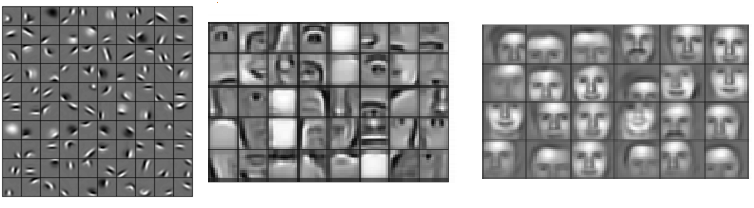
\includegraphics[width=.85\linewidth]{hierarchical_features.png}
 \caption{Learned hierarchical feature learned by Deep Learning algorithm\cite{NvidiaConcepts}}
 \label{fig:FeatLearn}
 \end{center}
 \end{figure}

\section{Logistic Classifier}
The next two sections are going to explain the theory behind deep learning by starting with a logistic classifier and evolving it into a deep network.  The purpose of a logistic classifier is predict a categorical class, given input data.  \textit{Is this an image of a 5? or a 4?}

Throughout all of deep learning the fundamental ingredients are a) Data b) Structure c) Loss and d) Optimizer

\subsection{Data}
As with all supervised machine learning algorithms, it is important to split the data into three sets: training, validation, testing.  Normally, the data is split into 70\% training, 20\% validation, and 10\% testing.  

The training and validation sets are used during training.  The training set is used to adjust the weights of the model.  While the validation set does not update the weights, it is used to validate that the model is not overfitting.  \emph{Overfitting} is when a model is overly complex - it has superfluous freedom to align with the specific data.    

Overfitting can be seen in the following analogy.  A student, analogous to our network model, takes two exams of the same subject repeatedly.  Over many trials the student will improve.  However, if the student's accuracy increases on Test 1 but not on Test 2, then he may be memorizing the answers, not learning the material.  The same is true for our model.  It could be overfitting the training data and not learning the underlying relationship.

The test set is new, unseen data that is only used for testing the final model's predictive power.  To follow the student analogy, the test set is the real world.  

\subsection{Structure}
\subsubsection{Neuron or Node}
The basic building block of a network is the neuron or node (Fig \ref{fig:neuron}).  It takes some input data, applies a linear function to those inputs by calculating a weighted sum, and applies an activation function to that sum.    


\begin{figure}[!h]
 \begin{center}
 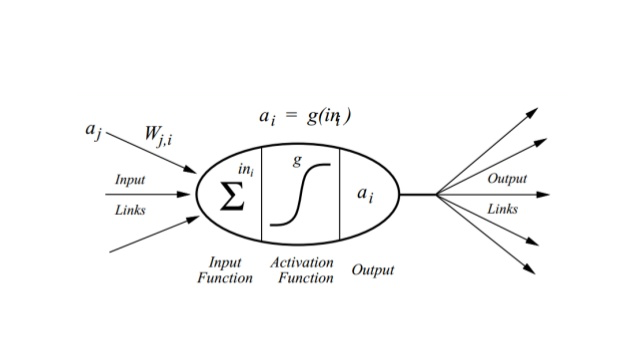
\includegraphics[width=.8\linewidth]{neuron.png}
 \caption{Neuron or node: Basic unit of Deep Learning}
 \label{fig:neuron}
 \end{center}
 \end{figure}
 
 The linear function is defined as 
\begin{equation}
WX+b = Y
\end{equation}
where $X$ denotes an input vector, $W$ denotes a matrix of weights, $b$ denotes the biases, and $Y$ denotes the \emph{scores} or \emph{logits}.  The training happens by trying to find the weights and biases that are good at predicting the correct class.  
For example, take a model that is trying to learn handwritten digits with an input as an image of a handwritten "5."  The linear function (Fig \ref{fig:Lin}) takes that input and outputs logits.  At first these outputs do not mean much.  The task is to determine the probability the image belongs to each class (digit).  The way to turn logits into probabilities is to apply a softmax as our activation function, see Fig \ref{fig:SftMax}.
\begin{figure}[!h]
 \begin{center}
 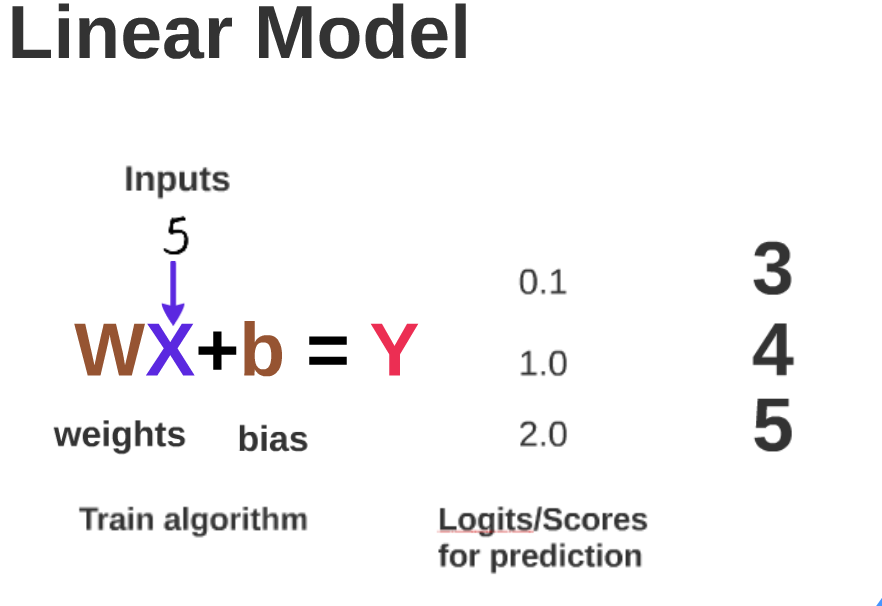
\includegraphics[width=.6\linewidth]{LinFunc.png}
 \caption{Linear Function }
 \label{fig:Lin}
 \end{center}
 \end{figure}
 
\begin{figure}[!h]
 \begin{center}
 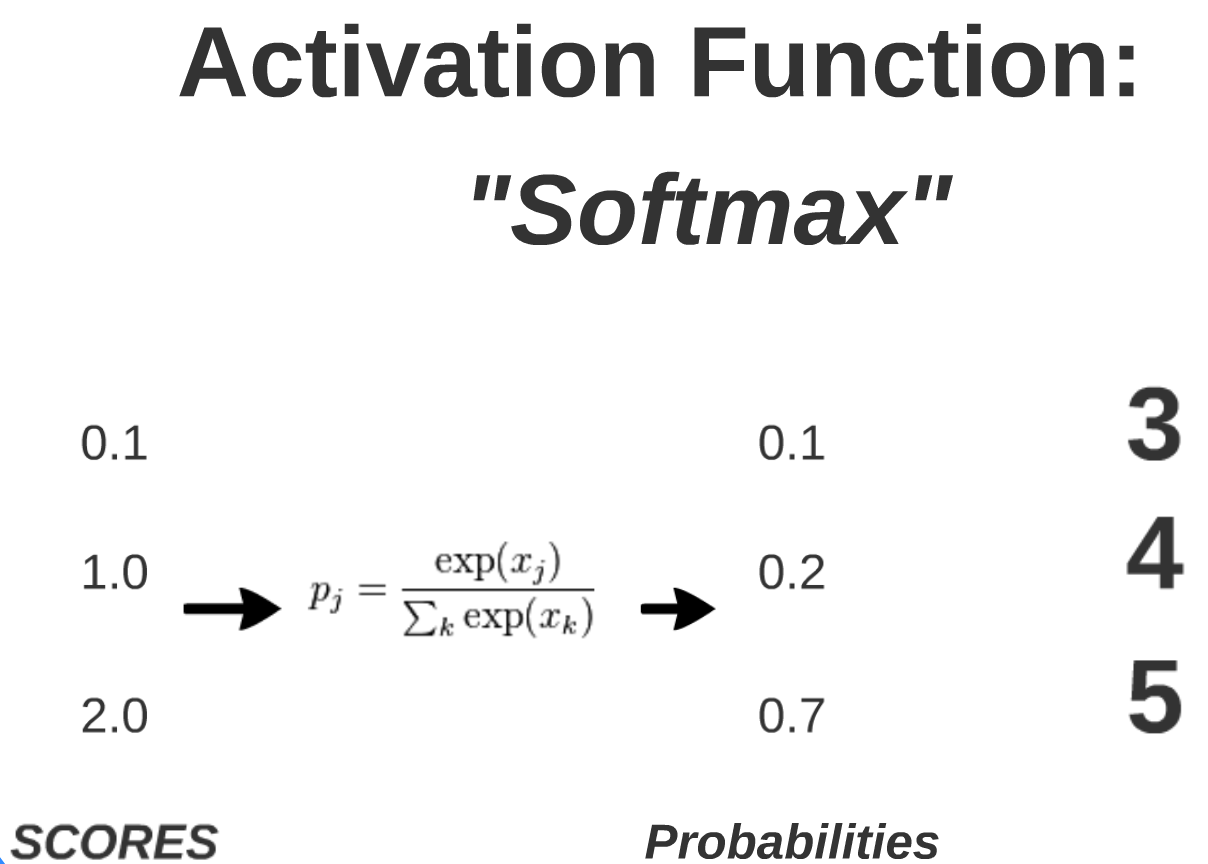
\includegraphics[width=.6\linewidth]{sftMax.png}
 \caption{To turn logits into probabilities, the activation function was chosen to be softmax}
 \label{fig:SftMax}
 \end{center}
 \end{figure}
 
The softmax function outputs the probabilities the image belongs to each class (the most likely is close to 1 and the less likely are close to 0).  The technique of One-hot Encoding is used to turn each label into a class-membership vector.  This vector has the value 1 for the correct class, and 0 for the rest of entries.  In the above example, the five is the correct label, so the one-hot encoded vector is [0,0,1]. 

There are now two vectors, one from the classifier (the probabilities) and one that represents the correct label (encoded vector). 

\subsection{Loss}
For the feedback in the model to work, there must be a metric of success.  The way to measure the distance between potential two vectors is called Cross Entropy, Eq \ref{Eq:X-entropy}. The goal is to have a low distance for a correct class but a high distance for an incorrect one.    
\begin{equation}\label{Eq:X-entropy}
D(S(Y),L)) = \sum_{k}^{ }L_{k}log(S(Y_{k})))
\end{equation}
The Training Loss, Eq \ref{Eq:TrainingLoss}, is defined as the average cross entropy over the entire training set ($i$). A good model has a low training loss.   

\begin{equation}\label{Eq:TrainingLoss}
\mathfrak{L} = \frac{1}{N}\sum_{i}^{ }D(S(WX_{i}+b)),L_{i})
\end{equation}
The loss is a function of the weights and the biases, so we are going to minimize that function using an optimizer.\cite{Udacity} 
\subsection{Optimizer}
One of the most popular optimizing techniques in machine learning is called Stochastic Gradient Descent (SGD).  It takes small steps along the loss surface following the gradient until it finds a minimum.  Recall the gradient is the multivariate slope of a function.  The size of the step is called the \emph{learning rate}.  The bigger the learning rate the faster it learns, but it may not reach the absolute minimal loss.  In practice, SGD is performed over multiple passes of the data set called epochs.  

SGD is popular in machine learning  because it scales well with data and model size.  However, it comes with additional hyper-parameters.  These are different from ordinary parameters that the model optimizes.  Examples of hyper-parameters that the user must tune are:
\begin{itemize}
\item Learning Rate initialization
\item Learning Rate decay
\item Weight initialization
\item Number of Epochs 
\end{itemize}

\subsection{Summary}
To summarize, we have created a linear model that outputs probabilities [structure].  We evaluate how the model is doing by calculating the cross entropy [loss] and use SGD [optimizer] to minimize that loss.  It is still a shallow model, but these are the fundamental tools for going deeper.   
% * <darren@myhigherground.com> 2016-05-19T04:06:28.296Z:
%
% > To summarize, we have created a linear model that outputs probabilities [structure].  We evaluate how the model is doing by calculating the cross entropy [loss] and use SGD [optimizer] to minimize that loss.  It is still a shallow model, but these are the fundamental tools for going deeper.   
%
% awesome paragraph.  give me that same thing in the beginning of the section as part of the intro so i get a better sense of where things are going.
%
% ^.

\section{Deep Learning}
\subsection{MultiLayer Perceptron [MLP]}
To turn the logistic classifier into a network, a second neuron is linked between the current neuron and the input (Fig \ref{fig:basic2L}).  This is called a two-layer Neural Network (the input layer is not counted).   

Layers are the highest level building block of a network.  The new layer is called the Hidden Layer because its output values are not visible to the network output.  The hidden layer gives the model the opportunity to represent the data in a simpler way.

The depth of the network is defined by the number of hidden layers. 

\begin{figure}[!h]
 \begin{center}
 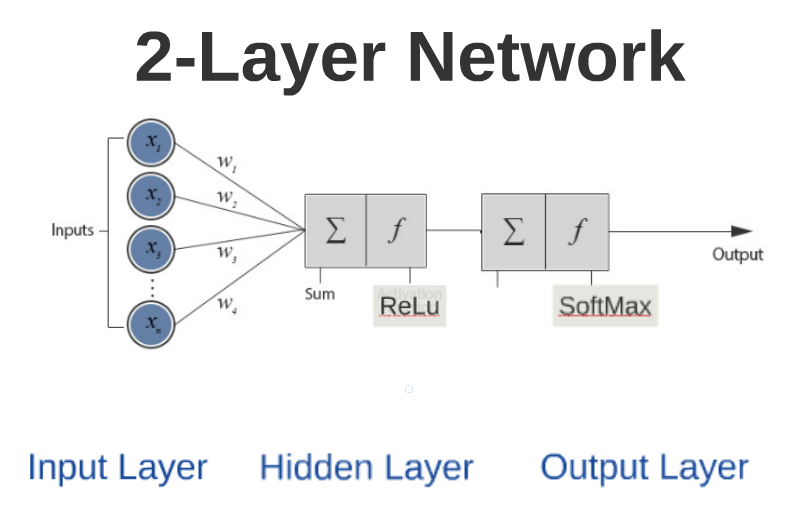
\includegraphics[width=.8\linewidth]{basic_2layer.png}
 \caption{Basic two layer Neural Network}
 \label{fig:basic2L}
 \end{center}
 \end{figure}
In addition to layers, the number of nodes per layer can increase as well.  The number of nodes on a layer represents the degree of freedom of that layer.  

When the output of every node on one layer is connected to the input of every node on the next layer, the network is called \emph{Fully Connected} or \emph{Dense}.  

The size of a network is defined by the number of layers and the number of nodes or parameters.  Fig \ref{fig:NN2} has 2 layers, 4+2=6 nodes (do not count input) or [3x4]+[4x2] = 20 weights and 4+2=6 biases for a total of 26  parameters.  Fig \ref{fig:NN3} has 3 layers, 9 nodes, and 42 learnable parameters.  

Modern convolutional neural networks have 100 million parameters and 20 layers (hence deep learning).  

\begin{figure}[!h]
\centering
\begin{subfigure}{.4\linewidth}
  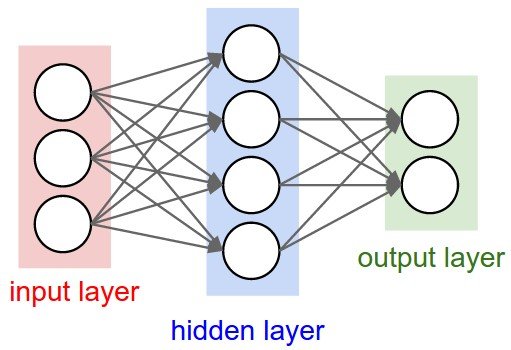
\includegraphics[width=\linewidth]{NN_2layer.jpeg}
  \caption{2-Layer}
  \label{fig:NN2}
\end{subfigure}%
\hfill
\begin{subfigure}{.6\linewidth}
  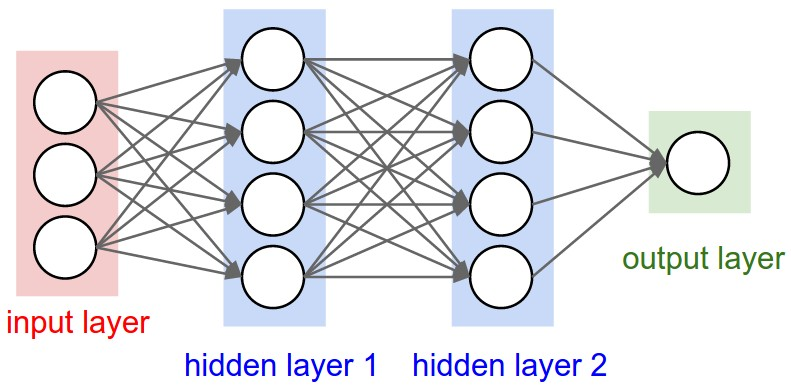
\includegraphics[width=\linewidth]{layerView.jpg}
  \caption{3-Layer}
  \label{fig:NN3}
\end{subfigure}
\caption{Two Fully connected Neural Networks\cite{Stanf}}
\label{fig:test}
\end{figure}

Evolving the structure from a single node into a network has allowed the model more opportunities to represent the data in a simpler way (layers) and more degrees of freedom (nodes).  However, the model is still linear. Because of superposition, stacking a 100 purely linear transformations can be simplified to a single layer. The solution is to introduce non-linear functions.

\subsection{Non-Linearities}
To preserve the network's structure (and the benefits gained with this structure), each hidden layer is given a non-linear activation function.  By adding non-linearity, the entire model is now non-linear and cannot be simplified down to a single transformation.  This creates a hierarchy of abstraction that grows in complexity with every layer.\cite{NvidiaConcepts} \cite{DataWknd}    


This is the foundation for building deep models.    


%Non-linear transformations increase the complexity of the relationships.  In DL, this creates increasingly complex features with every layer.  In contrast, stacking 100 purely linear transformations can be simplified to a single layer.  That is, even when multiple node layers are added, because of superposition, the layers can be rearranged into a single mapping.  For nonlinear layers, the mapping is non-separable - forcing different levels of complexity to be modeled.  
% * <darren@myhigherground.com> 2016-05-19T04:11:23.523Z:
%
% > Non-linear transformations increase the complexity of the relationships.  In DL, this creates increasingly complex features with every layer.  In contrast, stacking 100 purely linear transformations can be simplified to a single layer.\cite{NvidiaConcepts}  That is, even when multiple node layers are added, because of superposition, the layers can be rearranged into a single mapping.  For nonlinear layers, the mapping is non-separable - forcing different levels of complexity to be modeled.  This is the foundation for building deep models. 
%
% you should edit my sentance, but this is a SUPER important paragraph.  i didn't even think about how important this was until you pointed it out.  thats the whole reason its called deep.  neat
%
% ^ <nreis@ucdavis.edu> 2016-05-19T23:04:54.605Z.

There are multiple types of non-linear activation functions: softmax, sigmoidal/logistic, tanh, and the rectified linear unit [ReLU].  A ReLU is a very simple, very powerful non-linearity.  Its output is linear for x greater than zero and zero everywhere else (Fig \ref{fig:ReLU}). Since its introduction in 2012, ReLu has become the most popular non-linearity because it does not face gradient vanishing problems as with sigmoid and tanh function.\cite{DataWknd}


\begin{figure}[!h]
 \begin{center}
 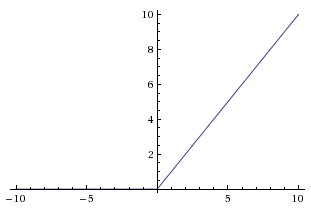
\includegraphics[width=.6\linewidth]{Relu.jpeg}
 \caption{Rectified Linear Unit is the most popular nonlinear function.  }
 \label{fig:ReLU}
 \end{center}
 \end{figure}

\subsection{Summary}
By constructing this MLP network we have given the model a better structure 
\begin{itemize}
\item Hidden Layers - number of moves to figure out a simpler way to represent the data
\item Number of nodes per hidden layer - the degrees of freedom for that move
\item Non-linearities allow increasing feature complexity with each layer  
\end{itemize}
We then told the network to learn the best parameters in order to correctly classify the input.
This is the core to Deep Learning.\cite{Udacity} \cite{DataWknd} \cite{playground}

\section{Convolutional Neural Networks}
Deep networks are powerful but can quickly increase in complexity.  Back to the example of classifying handwritten digits.  If the input image is 32x32 pixels with 3 colors and the network has 2 fully connected layers with 2 outputs (similar to Fig \ref{fig:NN2}) then there would be a total of 9.4 millions learnable parameters.  That is a lot of parameters for a small image and a simple structure.  To help out the model, the user can use his or her domain knowledge (the fact that it is an image).    

Take an image of a cat.  It does not matter where in the image the cat is, it is still an image of a cat.  This is called translational invariance.  Identifying invariant structure is a key aspect in machine learning because it is a direct path to efficient learning.  In a fully connected network, the model learns weights for cats in the right corner and different weights for cats in the left corner.  Instead, the user would like the model to learn features by sharing weights across the entire image.  This is called \emph{convolutions}.   
\subsection{Convolutions}
Fig \ref{fig:CNN} is an example of an input image ($X$)  with a cat in it.  The image has a width, height, and a depth (represented by the RGB colors).  Take a small patch of the image and run a tiny neural network on it with $k$ outputs.  Sliding that patch across the entire image creates a new image with a new width, height, and a depth of $k$.  If the patch was the size of the original image, it would be no different than a fully connected layer.  However, by sweeping a smaller patch across the image  there are fewer weights and the weights are shared across space.  

\begin{figure}[!h]
 \begin{center}
 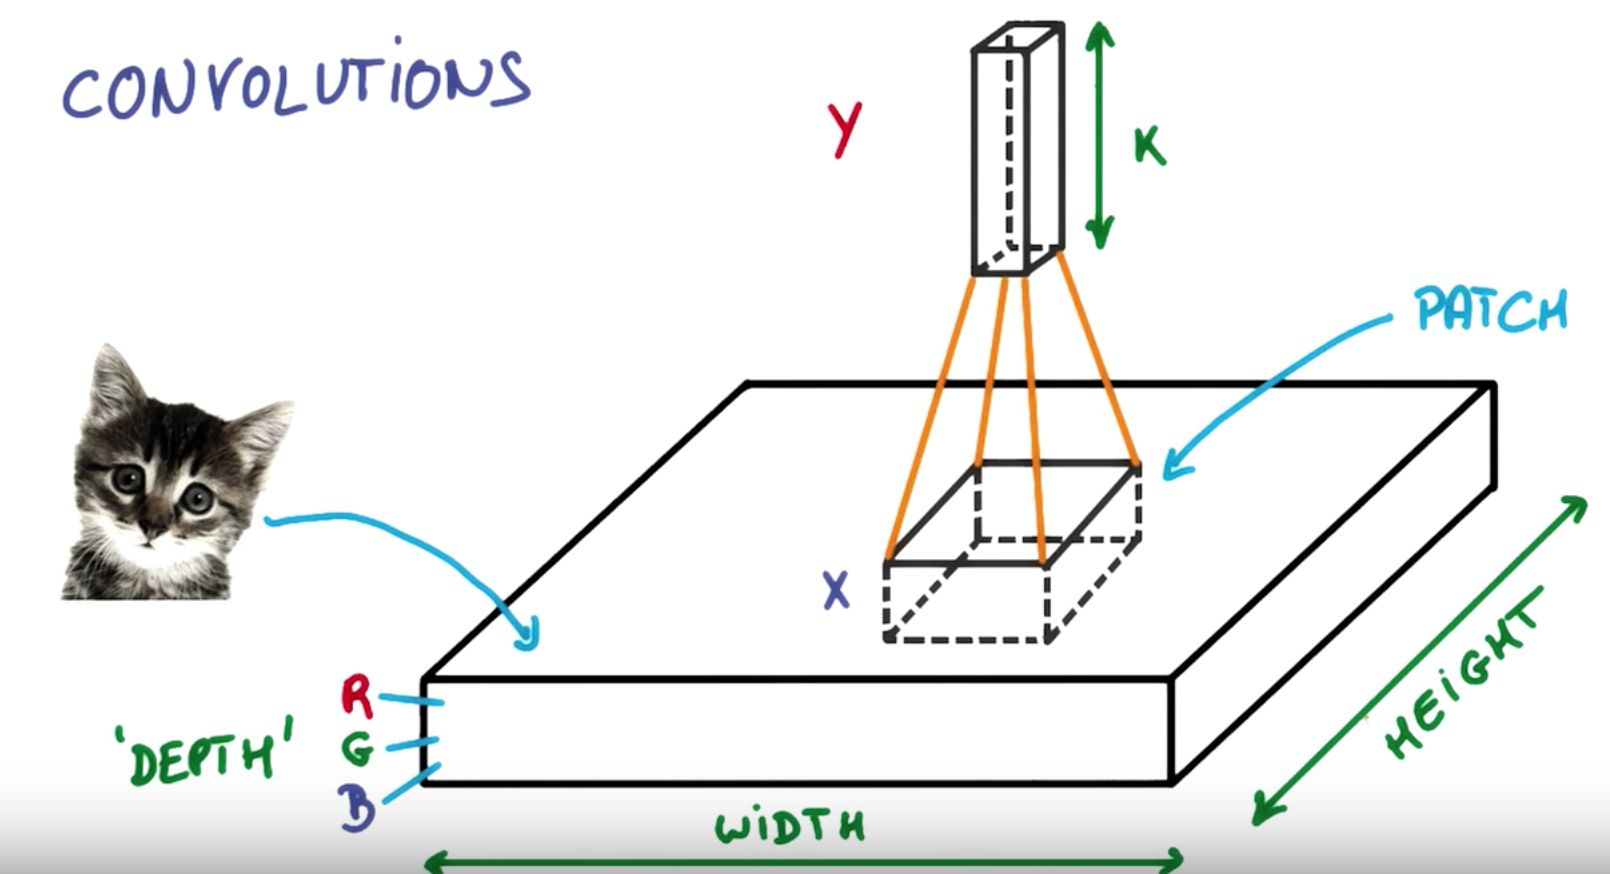
\includegraphics[width=.7\linewidth]{CNN.png}
 \caption{Sketch of how a Convolution passes over an image \cite{Udacity}}
 \label{fig:CNN}
 \end{center}
 \end{figure}

\subsection{Network}
Convolutions are stacked on top of each other to form a convolutional pyramid, Fig \ref{fig:ConvNet}.  The layers progressively squeeze the spatial dimensions, while increasing the network depth.  The depth can be thought of as the semantic representation.  At the end, a fully connected classifier is attached.  Through training, these convolutional layers form the hierarchy of abstraction seen in Fig \ref{fig:FeatLearn}. \cite{Udacity} \cite{DataWknd} 

\begin{figure}[!h]
 \begin{center}
 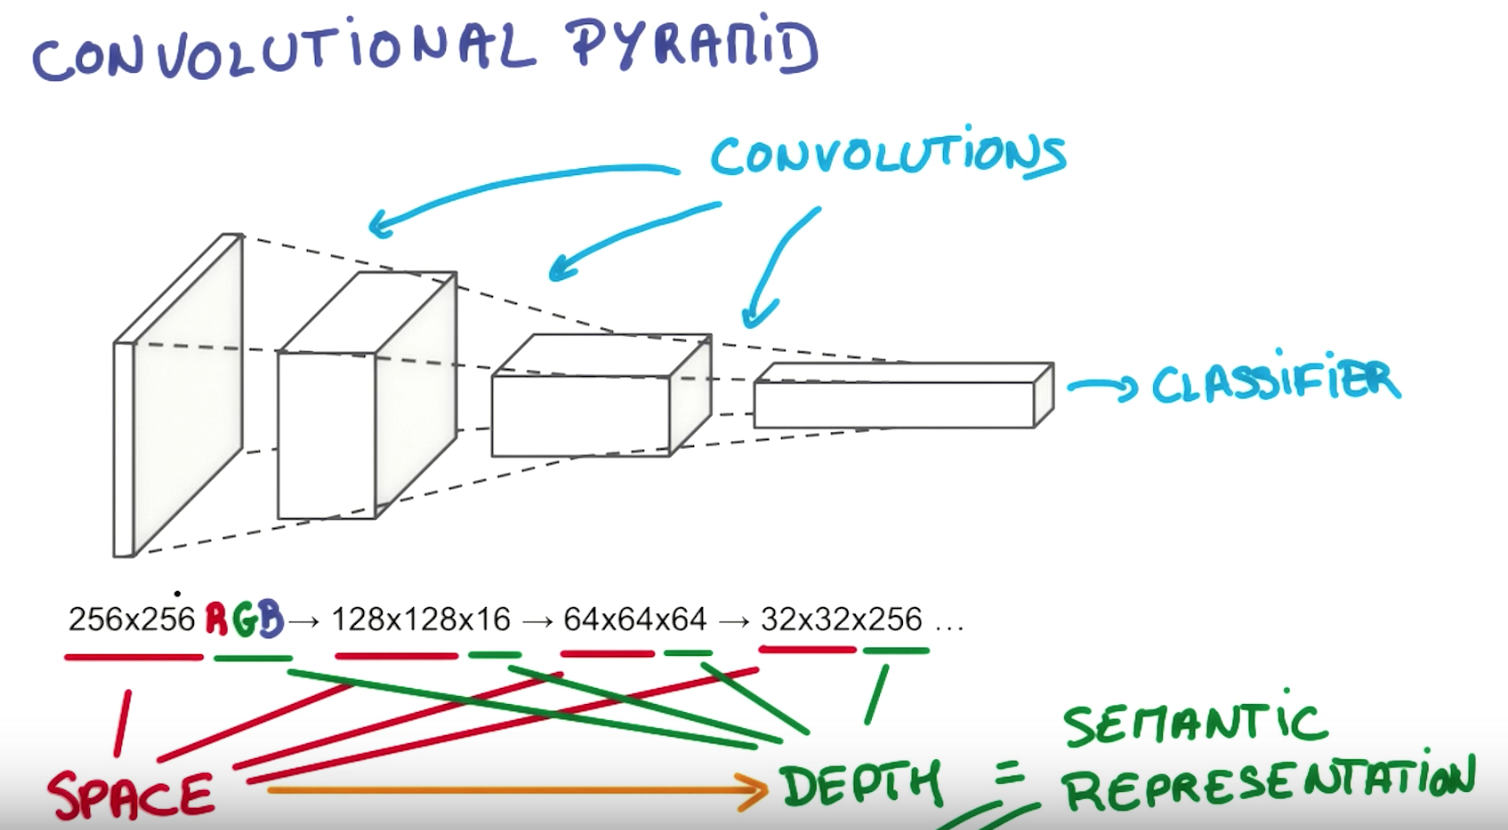
\includegraphics[width=.85\linewidth]{CNN_stack.png}
 \caption{Structure of a ConvNet \cite{Udacity}}
 \label{fig:ConvNet}
 \end{center}
\end{figure}

\section{Example: MNIST}
The challenge of classifying handwritten digits is a classic machine learning problem.  The dataset used is called MNIST and it was one of the first real world problems solved by neural networks.  
\subsection{Data}
MNIST contains 60,000 training images and 10,000 test images of handwritten digits from 500 different writers.  Each image is a grey scale 28x28 pixel image.  10\% of the training data was reserved for validation.  
\subsection{Structure}
Two structures were evaluated: MultiLayer Perceptron [MLP] and a ConvNet.
\subsubsection{MLP}
A 2-Layer Perceptron [MLP] was built with fully connected layers. The input was an image flattened to a vector of length 784 (28x28).  This input was fully connected to a hidden layer with 512 nodes with a ReLU activation function.  The hidden layer was fully connected to the output layer of length 10 (0-9) with a softmax.\footnote{Dropout was applied to combat overfitting}

\subsubsection{ConvNet}
The input image was kept in its original form 1x28x28.  It was inputted into two convolutional layers which squeezed it to a shape of 32x14x14.  That image was fed into the same MLP classifier as described above.
\subsection{Loss and Optimizer}
Both models defined the loss as cross entropy and used RMSprop as their optimizer.  [RMSprop is a version of SGD with an adaptive learning rate].
\subsection{Results}
The results are shown in the Table \ref{tbl:MNIST} below.  Both algorithms performed excellent. Out of the 10,000 test points, the MLP missed 188.  The  ConvNet misclassified only 93;  it was twice as accurate in half the number of epochs.  Fig \ref{fig:MNIST} shows the loss curves for each, demonstrating that neither model overfit the training data.  The time per epoch was listed because this example was done on the author's personal computer (2014 13in Macbook Pro running OS X 10.11.4, 2.6GHz 8GB, Intel Iris 1536MB).  At the time of purchase, the author had no intention of demanding more than basic performance from his machine.  Had this experiment been run on a GPU the training time would have been an order of magnitude faster.  


\begin{table}[h!]
\centering
\caption{Results from Classifying MNIST}
\label{tbl:MNIST}
\resizebox{\linewidth}{.3in}{%
\begin{tabular}{ccc|ccc}
\hline
\multicolumn{1}{l}{} & \multicolumn{1}{l}{} & \multicolumn{1}{l|}{} & \multicolumn{3}{c}{Accuracy}            \\ \hline
                     & Epochs               & time per Epoch [s]    & Training Set & Validation Set & Test Set \\ \cline{2-6} 
MLP                  & 10                   & 10                    & 0.9822       & 0.9828         & 0.9812   \\
CNN                  & 5                    & 360                   & 0.9928       & 0.9915         & 0.9907   \\ \hline
\end{tabular}%
}
\end{table}


\begin{figure}[!h]
\centering
\begin{subfigure}{.5\linewidth}
  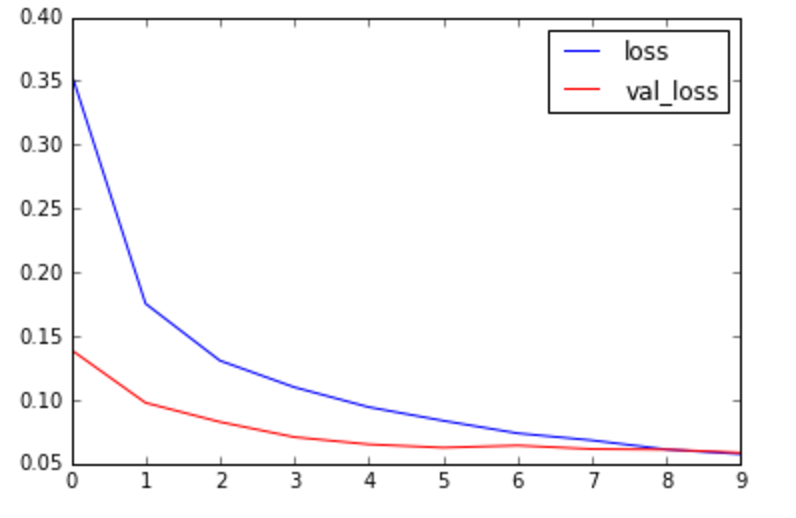
\includegraphics[width=\linewidth]{MLP.png}
  \caption{MLP}
  \label{fig:MLP}
\end{subfigure}%
\hfill
\begin{subfigure}{.5\linewidth}
  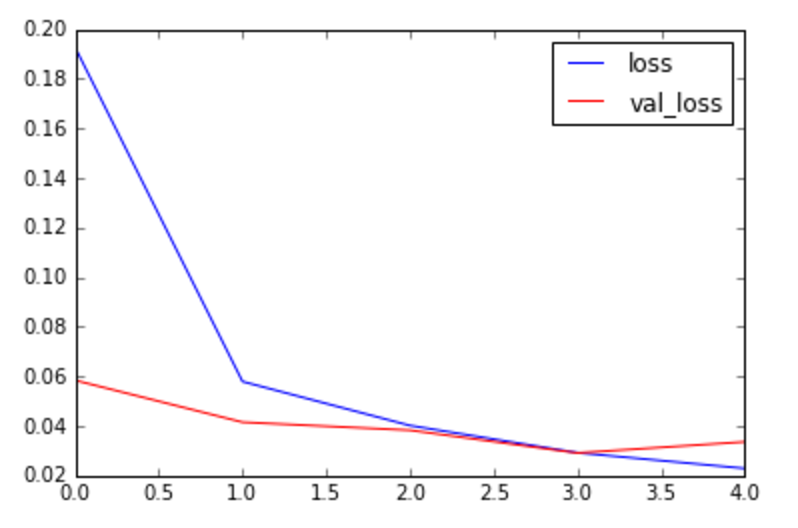
\includegraphics[width=\linewidth]{CNN_loss.png}
  \caption{ConvNet}
  \label{fig:NN3}
\end{subfigure}
\caption{Loss as a function of epoch.  The fact that the training and validation losses converge is evidence that the model is not overfitting}
\label{fig:MNIST}
\end{figure}

\section{Tools}
The good news is that the field of DL is exploding and a majority of it is open-source.  The bad news is that this field is in its infancy so there are a lot of options and it is difficult to configure your system.  
 
\subsection{Programming}
Deep learning is programmed in mostly Python or C++. Since it is just math, one can program all of the operations from scratch.  However, many common functions have been built into open-source toolkits.  The community has not consolidated yet, so there are over 50 different toolkits, each with its advantages and disadvantages.  The most popular include
\begin{itemize}
\item TensorFlow
\item Keras
\item Theano
\item Caffe
\item Torch
\item CNTK
\end{itemize}

Google open-sourced its toolkit called TensorFlow and it has gained a lot of traction in the six months since its release (November, 2015).  It is a very powerful toolkit that they are writing all of their algorithms on.  

The best place to start is a toolkit called Keras.  It is built to run on top of TensorFlow or Theano.  The purpose of this toolkit is to enable fast, easy prototyping.  While it is not as powerful as other options it allows beginners to get their hands dirty quickly. \footnote{It is this author's opinion that creating an environment inside anaconda was the most successful way to get started.}

In addition to toolkits, existing pre-trained networks are usually open-sourced.  Winning networks, such as AlexNet (the first ConvNet submitted to ImageNet), open-source their learned parameters and structure.  

\subsection{Transfer Learning}
One of the continuing limitations of DL is data.  While the amount of data is increasing exponentially, getting good, clean data is hard to come by.  Large corporations like Facebook or Google can pay for manual labeling of data, but everyone else uses shared data sets like MNIST over and over again.  Few DL models are trained from scratch.  It is logical to assume that is would stall innovation; however, this is not true.  It has been shown that CovNets learned from large data sets can learn generic features and be repurposed for other smaller databases. \cite{lin2015learning} 

\begin{figure}[!h]
 \begin{center}
 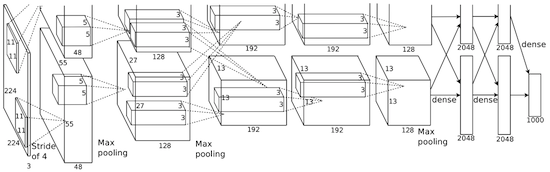
\includegraphics[width=.8\linewidth]{alexnet_small.png}
 \caption{The structure of AlexNet  \cite{AlexNet}}
 \label{fig:AlexNet}
 \end{center}
\end{figure}

\subsubsection{Fine Tuning}
Take a ConvNet pre-trained on ImageNet and cut off the last fully connected layer (that classifies the 1000 classes defined by ImageNet).  Retrain the CovNet by fine-tuning the existing weights for this new dataset. Essentially, the original weights are used as an initialization for the new task.  The motivation behind this strategy is that the lowest levels of the ConvNet contain generic features (edge detector or blob) that can be useful for many task; however, later layers become progressively more specific to the nuances of the classes for the original dataset.   For example, ImageNet has a number of dog breeds, so AlexNet likely has a number of later filters that can distinguish between the breeds. \cite{Stanf} 


\subsection{Technology}
As previously stated, the exponential rise in computational power has enabled DL to grow at an incredible rate.  In the 2000s, researchers recognized that the GPU inside gaming computers was perfect for quickly multiplying very large matrices.  They originally rode the rise of gaming computers, but lately, computer companies, like Nvidia, have taken notice of DL and begun building chips specifically designed for DL.  Deciding which GPU specifications is beyond the scope of this report but there are many resources for those who are interested. \cite{GPUs}  

Another option is Amazon Web Services [AWS].  A user can rent time on Amazon's GPUs to run an algorithm for a couple hours.  This is great for testing models out without the investment in hardware.  



